\section{توصيف الذراع الروبوتية}

تتكون الذراع الروبوتية المستخدمة في هذا المشروع من خمسة مفاصل دورانية (\LR{Revolute Joints})، مما يمنحها خمس درجات حرية (\LR{5-DOF})، وذلك دون احتساب حركة أداة النهاية (\LR{End-Effector}).

يبدأ تركيب الذراع بقاعدة ثابتة توفر الاستقرار للنظام، حيث يحتوي المفصل الأول على حركة دورانية حول المحور العمودي، مما يسمح بتغيير اتجاه الذراع في المستوى الأفقي. يرتبط بهذا المفصل مفصل ثانٍ يمثل حركة الكتف، والذي يتيح رفع وخفض الذراع في المستوى العمودي.

يتصل بالمفصل الثاني مفصل ثالث يمثل حركة الكوع، والذي يسمح بتمديد الذراع أو تقليصها للوصول إلى نقاط مختلفة ضمن مجال العمل. بعد ذلك، يوجد مفصلان إضافيان يشكلان جزء المعصم (Wrist)، حيث يساهمان في تحسين توجيه الذراع وضبط زاوية أداة النهاية.

يتم تشغيل جميع المفاصل باستخدام محركات سيرفو، مما يوفر دقة مناسبة في التحكم بزوايا المفاصل واستجابة سريعة للأوامر. وتعتمد الذراع على بنية تسلسلية، بحيث تؤثر حركة كل مفصل على الوضع النهائي لأداة النهاية.

تم تصميم هذه الذراع الروبوتية خصيصاً لتنفيذ مهام نقل الأجسام اعتماداً على الأوامر الصوتية، مما يتطلب نمذجة دقيقة للحركة باستخدام الحركيات الأمامية والعكسية، بالإضافة إلى دراسة الديناميك لفهم القوى المؤثرة أثناء التشغيل، كما هو موضح في الشكل \ref{fig:robot_arm}.

\begin{figure}[htbp]
\centering
\vspace*{\fill}
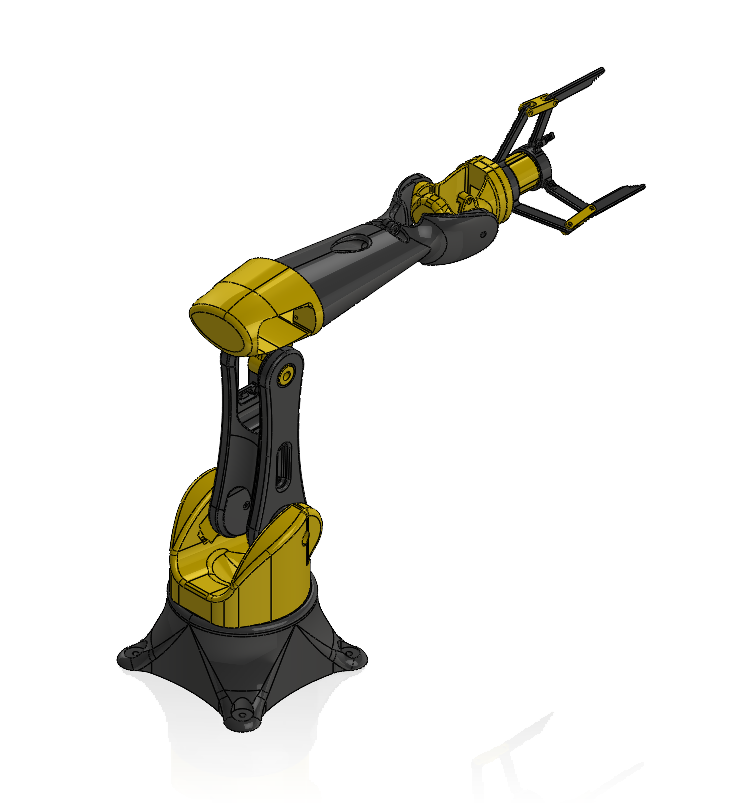
\includegraphics[width=0.8\textwidth]{resources/images/Assem1}
\captionof{figure}{\centering الذراع الروبوتية ذات خمس درجات حرية}
\label{fig:robot_arm}
\vspace*{\fill}
\end{figure}
